\documentclass[a4paper,12pt]{article}
\usepackage[T2A]{fontenc}
\usepackage[utf8]{inputenc}
\usepackage[english,russian]{babel}
\usepackage{amsmath,amsfonts,amssymb,amsthm,mathtools}
\usepackage{tikz}
\author{Баширов 778}
\title{Домашнее задание 10-11}

\begin{document}
\maketitle
\newpage
\noindent \large\textbf{1.1}\normalsize\\
Сложив потоки всех выходящих из истока ребер получаем поток равный 7.\\
\large\textbf{1.2}\normalsize\\
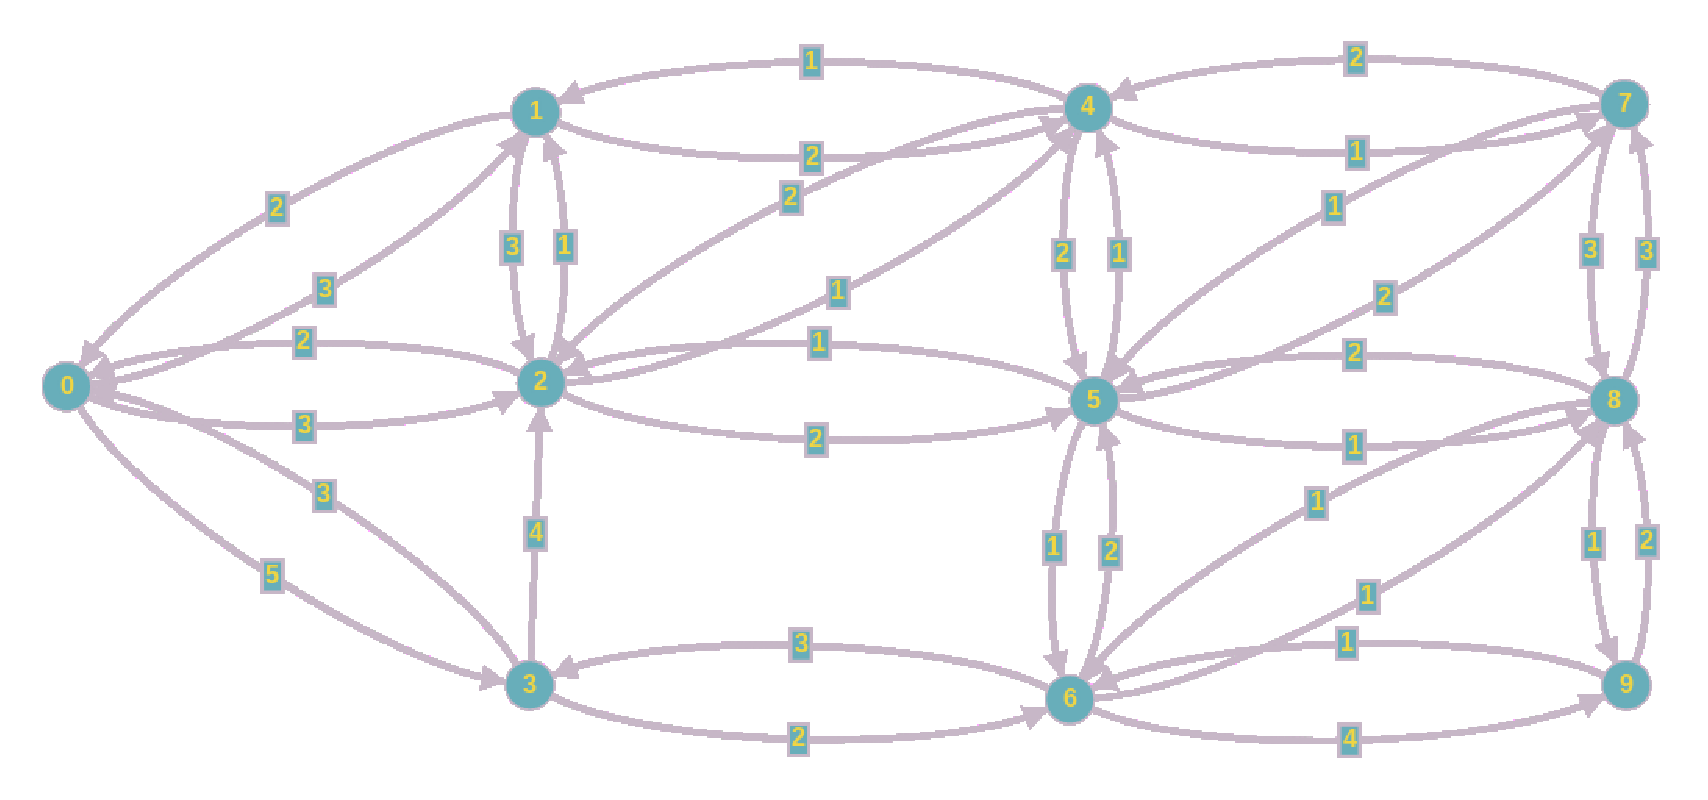
\includegraphics[scale=0.5]{image1}
\large\textbf{1.3}\normalsize\\
Поток не максимален так как в остаточном графе существует путь из s в t. Путь: 0, 1, 4, 7, 8\\
\large\textbf{4}\normalsize\\
На основе данной потоковой сети построим граф в котором можно найти максимальный поток по базавому алгоритму Форда-Фалкерсона. Для этого заменим все вершины кроме стока и истока на пару вершин соединенных ребром с весом равным пропускной способности исходной вершины. Замену произведем следующим образом: все ребра входившие в исходную вершину напрвим в первую вершину, все выходящие будут направлены из второй вершины, а новое ребро будет направлено из первой вершины во вторую. Все ребра которые входили в изначальный граф будут входить в новый граф с бесконечным весом. Веса ребер будут соответствовать пропускной способности. Итак, после переделывания графа осталось применить алгоритм Форда-Фалкерсона.\\
\end{document}